\documentclass{article}

% if you need to pass options to natbib, use, e.g.:
%     \PassOptionsToPackage{numbers, compress}{natbib}
% before loading neurips_2020

% ready for submission
% \usepackage{neurips_2020}

% to compile a preprint version, e.g., for submission to arXiv, add add the
% [preprint] option:
%     \usepackage[preprint]{neurips_2020}

% to compile a camera-ready version, add the [final] option, e.g.:
%     \usepackage[final]{neurips_2020}

% to avoid loading the natbib package, add option nonatbib:
     \usepackage[final, nonatbib]{neurips_2020}

\usepackage[utf8]{inputenc} % allow utf-8 input
\usepackage[T1]{fontenc}    % use 8-bit T1 fonts
\usepackage{hyperref}       % hyperlinks
\usepackage{url}            % simple URL typesetting
\usepackage{booktabs}       % professional-quality tables
\usepackage{amsfonts}       % blackboard math symbols
\usepackage{nicefrac}       % compact symbols for 1/2, etc.
\usepackage{microtype}      % microtypography
\usepackage{float}
\usepackage{graphicx}
\usepackage{amsmath}


\title{ECSE 551 Mini Project 1}

% The \author macro works with any number of authors. There are two commands
% used to separate the names and addresses of multiple authors: \And and \AND.
%
% Using \And between authors leaves it to LaTeX to determine where to break the
% lines. Using \AND forces a line break at that point. So, if LaTeX puts 3 of 4
% authors names on the first line, and the last on the second line, try using
% \AND instead of \And before the third author name.

\author{
  Isabel Lougheed,~260989364 \\
  \And
  Mathieu Mailhot,~260989370 \\
  \And
  Frank-Lucas Pantazis,~260986139 \\
  % examples of more authors
  % \And
  % Coauthor \\
  % Affiliation \\
  % Address \\
  % \texttt{email} \\
  % \AND
  % Coauthor \\
  % Affiliation \\
  % Address \\
  % \texttt{email} \\
  % \And
  % Coauthor \\
  % Affiliation \\
  % Address \\
  % \texttt{email} \\
  % \And
  % Coauthor \\
  % Affiliation \\
  % Address \\
  % \texttt{email} \\
}

\makeatletter
\renewcommand{\@noticestring}{}  % Removes footer text
\makeatother

\begin{document}

\maketitle

\begin{abstract}
  This project involves implementing a logistic regression linear classifier from scratch.  This report presents the results of the logistic regression classifier model when performed on two datasets, a Chronic Kidney Disease (CKD) dataset and a battery dataset.  Multiple logistic regression models were compared with training/validation data.  For the CKD dataset, a third-degree model was chosen and resulted in an error of 0.1250 using test data. For the battery dataset, a linear model where some features are removed was chosen and resulted in an error of 0.0508 using test data. 
\end{abstract}

\section{Introduction}

Machine learning is revolutionizing industries by providing powerful solutions to real-world issues. As its applications continue to grow, mastering this skill is becoming essential for professionals across various fields. The project focuses on developing a two-class classification model using a logistic regression classifier to address two key challenges: detecting chronic kidney disease (CKD) in patients and identifying defective batteries in a manufacturing plant. 
The datasets were split into a training/validation set consisting of approximately 90 \% of the data and a testing set that consisted of approximately 10 \% of the data.  Five different models were compared for each dataset.  Cross validation was performed on a linear model that included all normalized features, a linear model that included all standardized features, a linear model with some features removed, a quadratic model where some features have a quadratic term, a cubic model where some features have a cubic term added.  After cross-validation, the cubic CKD model and the feature removed battery model had the lowest error.  After testing these models on the separated testing data, the cubic CKD model resulted in an error of 0.1250 and the feature removed battery model resulted in an error of 0.0508. 

\section{Datasets}


The first dataset used is a CKD dataset. It has 330 samples, each containing 28 unlabeled and un-normalized numerical features which could be used to detect CKD in patients.  There is one target variable indicating whether the patient was diagnosed with CKD or not diagnosed with CKD. The dataset contains the same number of individuals having CKD as normal individuals. This number amounts to 165 persons with CKD and 165 persons without CKD. The distribution of each feature was analyzed, however no insight to help inform our interpretation of the data was found. From the distribution of each feature, no outlier data was found. No bimodal distribution and no uniform distribution were observed. Therefore, the number of features were altered based on the significance of the final weights of our model trained with the normalized data set.  From the weights of a linear model with all features included, feature 2 held the highest weight and therefore we added a higher order term for feature 2 in some of the models.  Features 3, 5, 14, 18, 21, 24, 25, 26, and 27 held the lowest weight and were therefore dropped in one of the models 
\\
\\
The second dataset used in this project is a battery dataset. It is comprised of 732 samples, each containing 32 unlabelled and unnormalized numerical features which could help identify defective batteries.  There is a target variable to classify whether the battery is normal or defective. The dataset contains the same number of defective batteries as normal batteries which amounts to 366 for each. From the distribution of each feature, no outlier data was found. For the same reason of not observing any bimodal distribution or uniform distribution as in the CKD data set, we decided to base our decision of removing features and adding features on the weight for each feature when training with the normalized data set, rather than base ourselves on the statistical analysis.  From the weights of a linear model with all features included, feature 1 held the highest weight and therefore we added a higher order term for feature 1 in some of the models.  Features 4, 19, 22, 25, and 27 held the lowest weight and were therefore dropped in one of the models 
\\
\\
Additionally, due to the high condition number of both datasets, which is when the dataset's features have very different magnitudes, the data should be normalized or standardized before learning a model. 

\begin{table}[ht]
  \centering
  \caption{Condition Number}
  \begin{tabular}{|c|c|c|}
  \hline
  \textbf{Condition} & \textbf{CKD Dataset} & \textbf{Battery Dataset} \\
  \hline
  Initial      & 1167.8498903169616 & 3154.5001615200767 \\
  Normalized   & 16.423607138042684 & 17.72325998977123 \\
  Standardized & 1.727045411594891  & 1.719599037744385  \\
  \hline
  \end{tabular}
  \end{table}

\section{Results}
\subsection{Hyperparameter Analysis}

The optimization of our models was achieved by testing different Gradient descent variations as well as fine tuning each model’s hyperparameters.  
\\
\\
For starters, two variations of gradient descent were implemented on the normalized CKD and battery datasets, using all available features. Since most of the models that we developed were trained on similar datasets (variations on the normalized dataset with all features), it seemed reasonable to assume that the best-performing gradient descent variation on this dataset would also perform well on the others. 
\\
\\
These two variations were: 
\begin{itemize}
  \item Gradient Descent with a Decaying Learning Rate [1]
  \item Momentum Based Gradient Descent [2]  
\end{itemize}
Although both models performed similarly in terms of accuracy, the gradient descent with a decaying learning rate converged with a much lower tolerance than momentum-based gradient descent. This suggests that it may be more precise. 
\\
\\
Following this, the step size for the decaying gradient descent for each model was fine-tuned by iterating through the following range of values [0.1, 0.011] and plotting its accuracy against its speed. Since our gradient descent method’s learning diminishes after each iteration, starting with larger step size values such as 0.1 is a better approach.  
\\
\\
By analyzing the performance of each model, it was determined that they all worked best with a starting step size of 0.03 and a tolerance of $10^{-6}$. As shown in figures 1 to 10 in the Appendix, the 1-accuracy value remained relatively constant across a wide range of step sizes. To distinguish the best-performing step size, convergence speed became the key criterion.  Indeed, when using larger step sizes, the convergence speed of the logistic regression was slower, and during the first iterations, the values tended to oscillate much less compared to smaller step sizes. Moreover, removing or altering feature values do not seem to affect performance speed at all. 

Although both models performed similarly in terms of accuracy, the gradient descent with a decaying learning rate converged with a much lower tolerance than momentum-based gradient descent. This suggests that it may be more precise.
\\
\\
Following this, the step size for the decaying gradient descent for each model was fine-tuned by iterating through the following range of values [0.1, 0.011] and plotting its accuracy against its speed. Since our gradient descent method’s learning diminishes after each iteration, starting with larger step size values such as 0.1 was a better approach.
\\
\\
By analyzing the performance of each model, it was determined that they all worked best with a starting step size of 0.03 and a tolerance of \( 10^{-6} \). As shown in the figures below, the \( 1 \)-accuracy value remained relatively constant across a wide range of step sizes. To distinguish the best-performing step size, convergence speed became the key criterion. Indeed, when using larger step sizes, the convergence speed was slower, and during the first iterations, the values tended to oscillate much less compared to smaller step sizes.
\\
\\
\subsection{Linear Model With All Features}

The first model that was implemented was a linear model that included data from all the features.  From the hyperparameter analysis, it was concluded that this model should be implemented with gradient descent with a step size of 0.03, a tolerance of $10^{-6}$, and an initial guess of 1 for each of the weights.  Through a 10-fold cross validation, the linear model using normalized data was compared to the linear model using standardized data.  It can be seen in tables 2 and 3 that the CKD linear model using normalized data performed better than with standardized data and the battery linear model using normalized data performed very similar compared to with standardized data.  Therefore, normalized data was used for all preceding models that were cross validated. 


\subsection{Removed Feature Model}
A model that is explored in this project is a model where some of the features are removed which we are naming feature removed model for the sake of this report. This model was implemented by calculating all the weights of the normalized model and then adding a threshold on the weights of each feature. The features that had a weight value below the threshold were simply removed.  Subsequently, the model was trained without those features. The threshold was found by iterating with a pressingly high value until the accuracy started to lower. It is also important to note that the data set has been normalized before the training. This is the reason why the weights of the features can be compared since they all are on the same basis. For the CKD data set, the threshold found that yields the best performance in terms of error is 0.1. This leads to removing features 3, 5, 14, 18, 21, 24, 26, and 27. With this model, the error is found to be 0.1215. For the battery data set, the threshold value that outputs the best accuracy performance is found to be 0.05.  This leads to removing features 4, 19, 22, 25, and 27. This lowers the error to 0.0508. One of the main reasons for implement this model or a variant of this model is its efficiency. Indeed, reducing the number of features will in many cases reduce the complexity of the model and in turn decrease the computational time to train the model. 

\subsection{Quadratic Model}

One of the models explored in this project is a quadratic model.  This was implemented by adding a quadratic term to the learned function for the more important features, the features with the highest weights attributed to them from the regular linear model.  For the chosen important features $x_i$, 
\begin{equation}
   f_w(x) = w_0 + w_1 x_i + w_2 x_i^2 + \dots
\end{equation}

A cross validation was performed on the quadratic model for each of the datasets for different amounts of quadratic features.  As seen in figures 11 and 12, 
as the number of quadratic terms increases, the error increases.  Therefore, for both the CKD quadratic model and the battery quadratic model, only one feature has a quadratic term in the learned function.   
Since the weights of the CKD linear model are 
\begin{equation*}
  \begin{aligned}
    [-1.0179,  2.4871, -0.0185,  0.1225, 0.0509,  0.1222, -0.2118, -0.2312, -0.3058, -0.1395, \\
    0.1897,  0.4275,  0.1648, -0.1032, -0.2050,  0.2870,  0.2827,  0.0557, 0.1185,  0.1652, \\
    -0.0089, -0.3447, -0.2880,  0.0708, 0.0002, -0.0845, -0.0942,  0.1653, -0.7693],
  \end{aligned}
\end{equation*}
the feature that has the largest weight magnitude, excluding  the bias weight is feature 2 and therefore feature 2 has a quadratic term.   
Since the weights of the battery linear model are 
\begin{equation*}
  \begin{aligned}
    [5.5288, 5.4114, -0.0814, 0.0036, 0.0838, -0.3571, -0.9275, -0.8126, -0.2352, -0.0839, \\
    -0.1379, -0.2578, -0.0698, -0.5288, -0.3349, -0.5354, -0.2542, -0.2727, -0.0385, -0.1533, \\
    -0.1472, 0.0454, 0.1609, 0.1094, 0.0360, -0.7155, 0.0190, -0.6298, -0.4767, -0.3815, \\
    -0.3547, -0.3608, -1.6986],
  \end{aligned}
  \end{equation*}
the feature that has the largest weight magnitude, excluding the bias weight is feature 1 and therefore feature 1 has a quadratic term. 

\subsection{Cubic Model}

To further expand the model, a cubic model was also tested.   The implementation of the cubic model is very similar to the quadratic model, except the more important features have polynomial terms of degree three in the learned function.  For the chosen important features $x_i$,
\begin{equation}
  f_w (x) = w_0 + w_1 x_i + w_2 x^2_i + w_3 x^3_i + \dots
\end{equation}
A cross validation was performed on the cubic model for each of the datasets for different amounts of cubic features.  
As seen in figures 13 and 14, as the number of cubic terms increases, the error increases.  Therefore, for both the CKD cubic model and the battery cubic model, only one feature has a cubic term in the learned function.  
This means that for the CKD cubic model, feature 2 has a cubic term and for the battery cubic model, feature 1 has a cubic term. 

\subsection{Cross Validation}

As seen in table 2, the cubic CKD model had the lowest error and therefore, the cubic CKD model is the final chosen model for the CKD dataset.  As seen in table 3, the feature removed battery model had the lowest error and therefore, the feature removed battery model is the final chosen model for the battery dataset. 

\begin{table}[h!]
  \centering
  \caption{Cross validation of different CKD models}
  \begin{tabular}{|l|l|l|}
  \hline
  \textbf{CKD Model}                               & \textbf{MSE}                  & \textbf{Error}               \\ \hline
  Linear model with all normalized features        & 0.21073183686528782           & 0.16896551724137931          \\ \hline
  Linear model with all standardized features      & 0.21760510560452745           & 0.1724137931034483           \\ \hline
  Feature removed model                            & 0.20451703420745432           & 0.16896551724137934          \\ \hline
  Quadratic model                                  & 0.20873582936775956           & 0.15862068965517245          \\ \hline
  Cubic model                                      & 0.2078159785211106            & 0.15517241379310348          \\ \hline
  \end{tabular}
\end{table}

\begin{table}[h!]
  \centering
  \caption{Cross validation of different battery models}
  \begin{tabular}{|l|l|l|}
  \hline
  \textbf{Battery Model}                            & \textbf{MSE}                  & \textbf{Error}               \\ \hline
  Linear model with all normalized features         & 0.0886492622549294            & 0.05846153846153843          \\ \hline
  Linear model with all standardized features       & 0.0886183051677138            & 0.05846153846153843          \\ \hline
  Feature removed                                   & 0.08827856579069857           & 0.05076923076923075           \\ \hline
  Quadratic model                                   & 0.08897472474905832           & 0.05846153846153843          \\ \hline
  Cubic model                                       & 0.08894956726027695           & 0.05846153846153843          \\ \hline
  \end{tabular}
\end{table}

\section{Discussion and Conclusion}

After cross validation, it was found that the cubic model resulted in the lowest error for the CKD dataset at 0.1552 and the feature removed model resulted in the lowest error for the battery dataset at 0.0508.  After testing these models on the testing data, it was found that the CKD cubic model resulted in an error of 0.125 and the battery feature removed model resulted in an error of 0.0508. 
\\
\\
A further direction for this project could be to test a model that removes irrelevant features and adds a quadratic or cubic term for more important features.  This new model would likely perform well for the CKD dataset since the feature removed, quadratic, and cubic models all outperformed the linear model with all features.  Whereas with the battery dataset, this new model would most likely not outperform the feature removed model since the quadratic and cubic models performed worse than the linear model with all features.  Nonetheless, it would be an interesting investigation. 

\section{Statement of Contributions}

Every team member contributed a fair share to the project. Frank-Lucas Pantazis worked on the fit, accu-eval, and predict methods of the project as well as optimizing the gradient descent with a momentum-based gradient descent. Isabel Lougheed worked on the normalization of the data, cross-validation, and developing the quadratic and cubic models. Mathieu Mailhot worked on the statistical analysis, and on developing the models with removed features. 

\section{Appendix}

\begin{figure}[H]
  \centering
  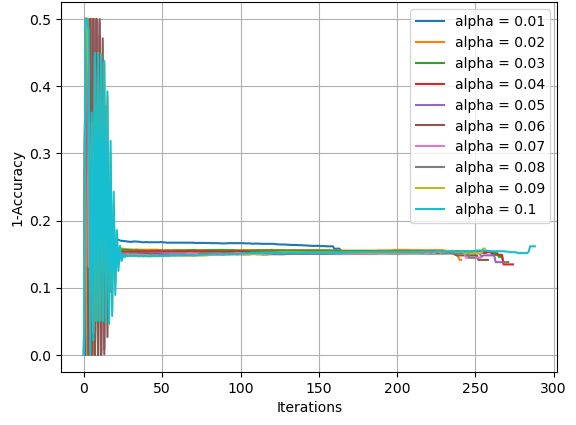
\includegraphics[width=0.8\textwidth]{CKDmodel1.png}
  \caption{Analysis of step size for CKD dataset with normalized features}
  \label{fig:quad_ckd}
\end{figure}

\begin{figure}[H]
  \centering
  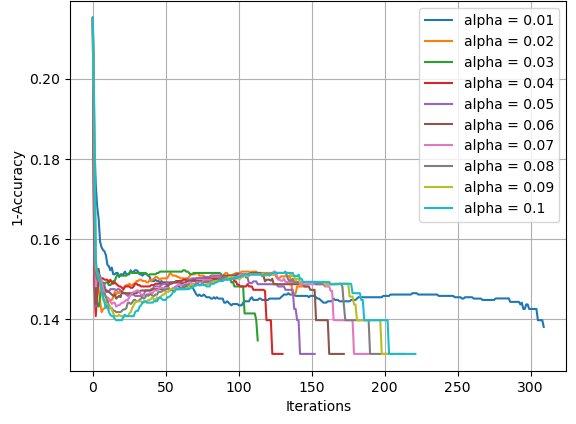
\includegraphics[width=0.8\textwidth]{CKDmodel2.png}
  \caption{Analysis of step size for CKD dataset with standardized features}
  \label{fig:quad_ckd}
\end{figure}

\begin{figure}[H]
  \centering
  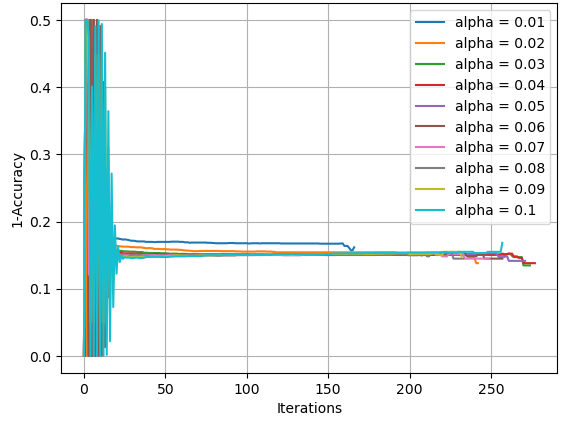
\includegraphics[width=0.8\textwidth]{CKDmodel3.png}
  \caption{Analysis of step size for CKD dataset with removed features model}
  \label{fig:quad_ckd}
\end{figure}

\begin{figure}[H]
  \centering
  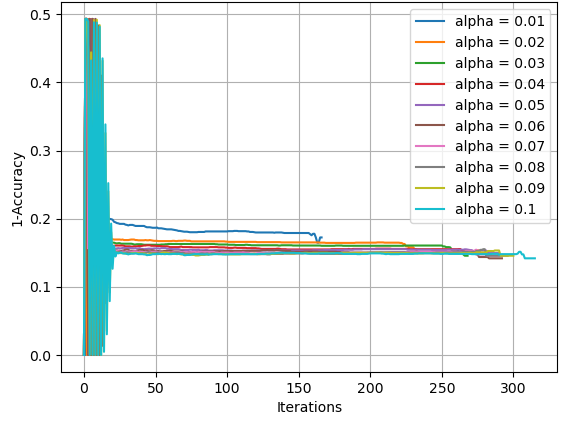
\includegraphics[width=0.8\textwidth]{CKDmodel4.png}
  \caption{Analysis of step size for CKD dataset with quadratic model}
  \label{fig:quad_ckd}
\end{figure}

\begin{figure}[H]
  \centering
  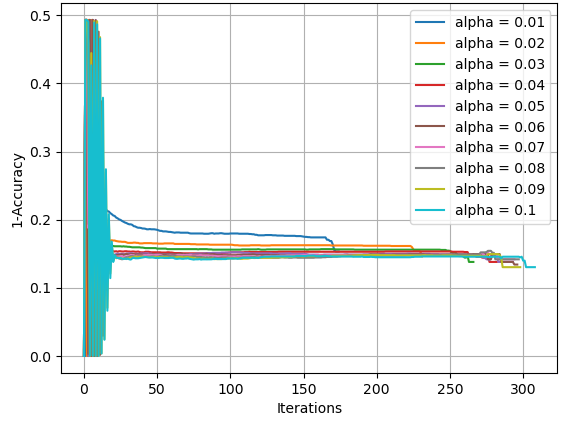
\includegraphics[width=0.8\textwidth]{CKDmodel5.png}
  \caption{Analysis of step size for CKD dataset with cubic model }
  \label{fig:quad_ckd}
\end{figure}

\begin{figure}[H]
  \centering
  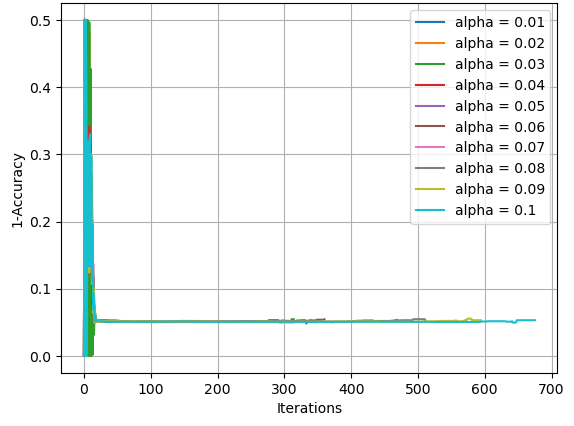
\includegraphics[width=0.8\textwidth]{Batmodel1.png}
  \caption{Analysis of step size for battery dataset with normalized features}
  \label{fig:quad_battery}
\end{figure}

\begin{figure}[H]
  \centering
  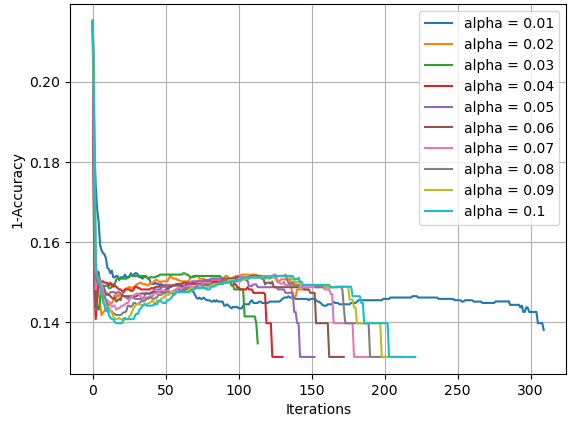
\includegraphics[width=0.8\textwidth]{Batmodel2.png}
  \caption{Analysis of step size for battery dataset with standardized features}
  \label{fig:quad_battery}
\end{figure}

\begin{figure}[H]
  \centering
  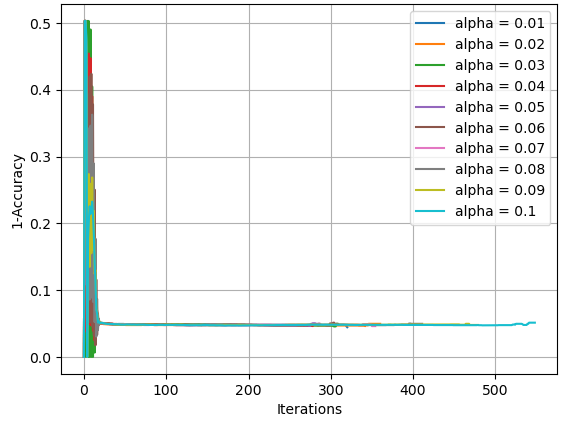
\includegraphics[width=0.8\textwidth]{Batmodel3.png}
  \caption{Analysis of step size for battery dataset with removed features model}
  \label{fig:quad_battery}
\end{figure}

\begin{figure}[H]
  \centering
  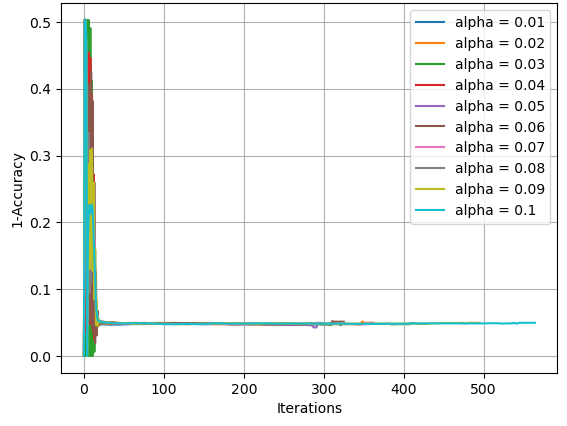
\includegraphics[width=0.8\textwidth]{Batmodel4.png}
  \caption{Analysis of step size for battery dataset with quadratic model}
  \label{fig:quad_battery}
\end{figure}

\begin{figure}[H]
  \centering
  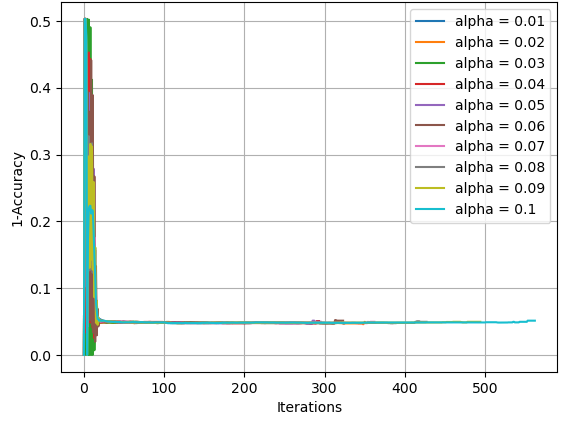
\includegraphics[width=0.8\textwidth]{Batmodel5.png}
  \caption{Analysis of step size for battery dataset with cubic model }
  \label{fig:quad_battery}
\end{figure}

\begin{figure}[H]
  \centering
  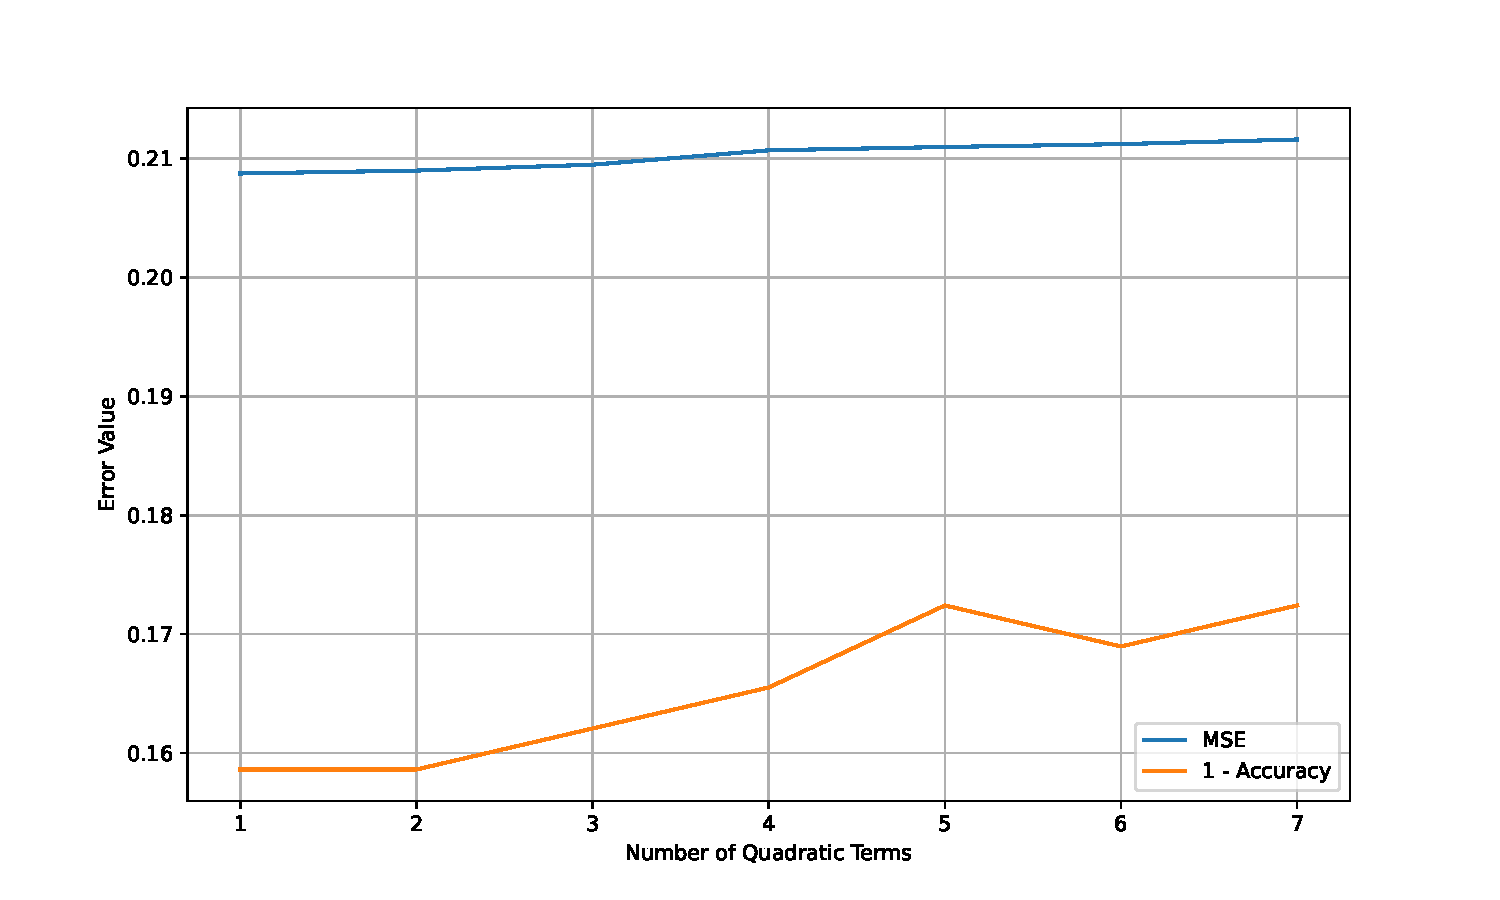
\includegraphics[width=0.8\textwidth]{quad_ckd.pdf}
  \caption{Number of quadratic terms vs. error for the CKD quadratic model}
  \label{fig:quad_ckd}
\end{figure}

\begin{figure}[H]
  \centering
  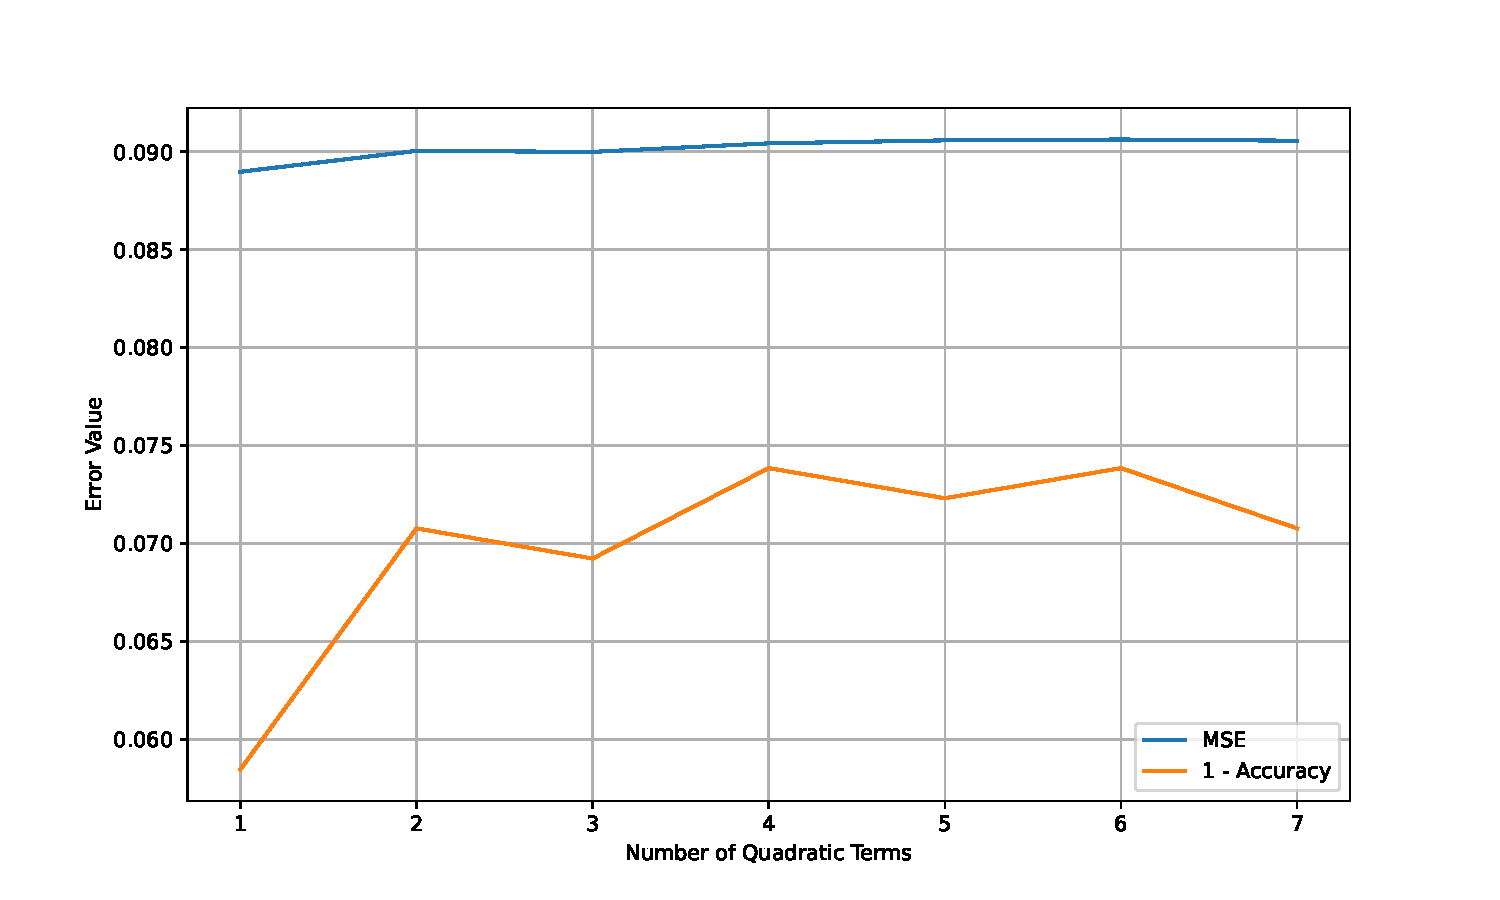
\includegraphics[width=0.8\textwidth]{quad_battery.pdf}
  \caption{Number of quadratic terms vs. error for the battery quadratic model}
  \label{fig:quad_battery}
\end{figure}

\begin{figure}[H]
  \centering
  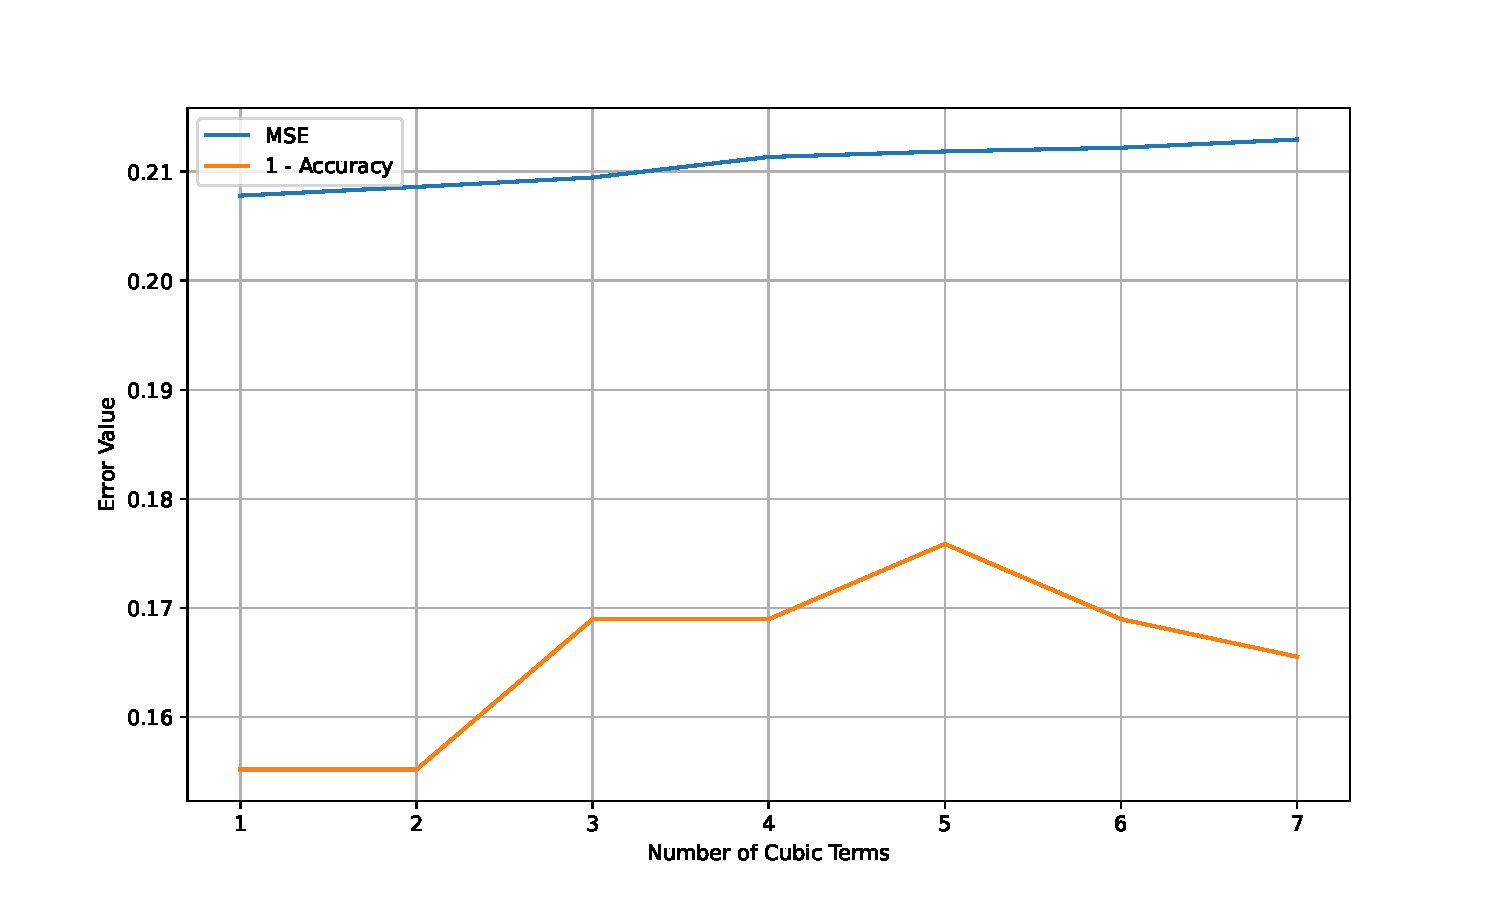
\includegraphics[width=0.8\textwidth]{cubic_ckd.pdf}
  \caption{Number of cubic terms vs. error for the CKD cubic model}
  \label{fig:quad_ckd}
\end{figure}

\begin{figure}[H]
  \centering
  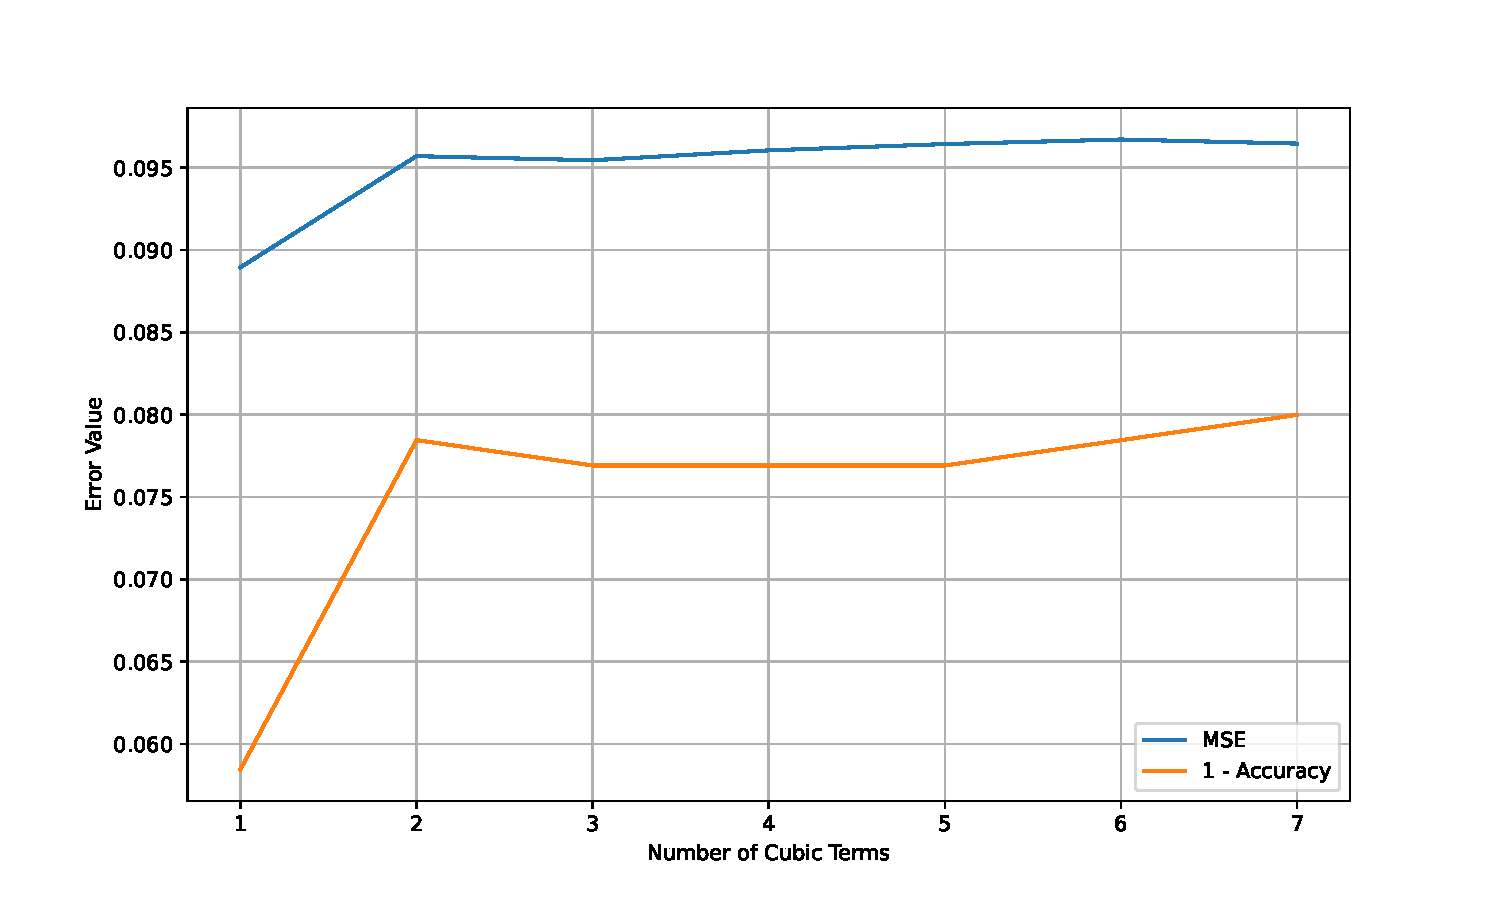
\includegraphics[width=0.8\textwidth]{cubic_battery.pdf}
  \caption{Number of cubic terms vs. error for the battery cubic model}
  \label{fig:quad_battery}
\end{figure}

\section*{References}

\medskip

\small

[1] Armanfard, N., (Winter 2025) ECSE 551: Machine Learning for Engineers, Electrical & Computer Engr, McGill University.

[2] GeeksforGeeks, “ML | Momentum-based Gradient Optimizer Introduction,” GeeksforGeeks, Feb. 15, 2019. [Online]. Available: https://www.geeksforgeeks.org/ml-momentum-based-gradient-optimizer-introduction/. [Accessed: Feb. 16, 2025].



\end{document}